\subsection{Hot Carrier Injection}

O fenômeno conhecido como \textit{Hot Carrier Injection} (HCI) vem sendo considerado uma preocupação no funcionamento de transistores MOS desde a década de 70 e vem sendo um dos efeitos de envelhecimento mais estudados desde então \cite{Butzen}.

A explicação clássica para o mecanismo físico desse efeitos é a geração de portadoras de alta energia devido a campos elétricos laterais elevados em transistores MOS quando estão no estado de saturação. Se essas portadoras ganharem energia suficiente podem ultrapassar a barreira de potencial e ser injetada no óxido do gate, causando danos na interface entre o óxido e o silício, aumentando a densidade de interfaces de estado e, consequentemente degradando parâmetros do componente, entre eles a tensão de \textit{treshold} \cite{Cacho}.

O HCI causa um impacto muito maior em transistores NMOS em comparação aos transistores PMOS devido ao fato da mobilidade de portadores do tipo n ser, de forma geral, maior do que a mobilidade de portadores do tipo p \cite{Jiang}.

A Figura \ref{fig:hci} mostra \textit{Hot Carriers} gerados por um alto campo elétrico lateral.

\begin{figure}[H]
    \centering
    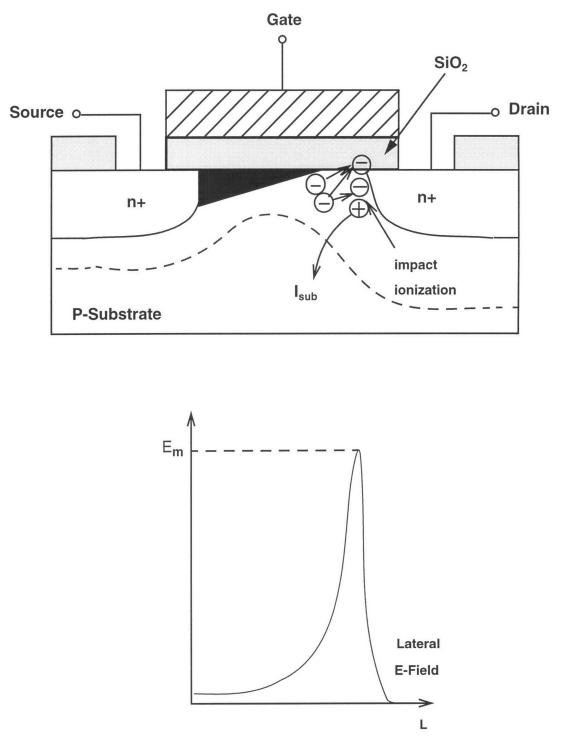
\includegraphics[scale=0.5]{figures/ReferencialTeorico/HCI.png}
    \caption{Geração de \textit{Hot Carriers} (acima) devido a um campo elétrico leteral (abaixo). Fonte: \cite{Jiang}}
    \label{fig:hci}
\end{figure}

